\chapter{Appendix \autoref{chap:vagram}}

\section{Full VAML for SAC}
\label{app:vagram:vaml_sac}
The formulation of VAML which we derive for SAC is a direct extension of the VAML loss to the SAC soft bellman backup. Specifically, given some distribution over the state-action space $\mathcal{D}$, state-action value function $Q$ and policy $\pi$, we can define a SAC-aware loss.

\begin{align}
    &\mathcal{L}_{Q, \pi}(\hat{p}, p, \mathcal{D}) = \nonumber\\
    &\quad \int \left|\int \left(\hat{p}(s'|s,a) - p(s'|s,a)\right) \E_{a' \sim \pi(\cdot| s')}{\left(Q(s', a') - \log \pi(a'|s')\right)} \mathrm{d}s'\right|^2 \mathrm{d} \mathcal{D}(s,a)\\
    &= \int \bigg|\int \left(\hat{p}(s'|s,a) - p(s'|s,a)\right) V^\pi(s', a')\mathrm{d}s' \nonumber\\
    &\quad\quad\quad- \int \left(\hat{p}(s'|s,a) - p(s'|s,a)\right)\mathbb{E}_{a' \sim \pi(\cdot| s')}\left[\log \pi(a'|s')\right] \mathrm{d}s'\bigg|^2 \mathrm{d} \mathcal{D}(s,a)
\end{align}
as well as its sample-based version:
\begin{align}
    &\hat{\mathcal{L}}_{Q, \pi}(\hat{p}, p, \mathcal{D}) = \sum_{i} \bigg|V^\pi(s_i') -\int \hat{p}(s'|s_i, a_i) V^\pi(s') \mathrm{d}s' - \nonumber\\&\quad\quad\left(\int \pi(a'|s_i')\log\pi(a' | s_i') \mathrm{d}a'- \int \int \hat{p}(s'|s_i,a_i)\pi(a'|s')\log\pi(a' | s')\mathrm{d}a' \mathrm{d}s' \right)\bigg|^2\label{SACVAMLLoss}
\end{align}

We find that in most of our experiments, the entropy terms did not significantly contribute to the loss. 
Therefore we dropped it in our experiments and directly derived VAGraM for the value function prediction error only.
This makes our loss applicable in all situations were the model is used to estimate the value function of a policy.

Finally, we do not account for the dependency of the policy function update on the model.
Since SAC aims to minimize the KL divergence between the action distribution and the Gibbs distribution defined by the value function directly, the only way the model influences this update is via the induced state space distribution.
We do not address this matching explicitly in this work, but a hybrid policy-aware and value-aware model is an enticing direction for future research.

\section{Additional experiments}

\subsection{Ablations}

\begin{figure}[t]
\begin{minipage}{.48\textwidth}
    \centering
    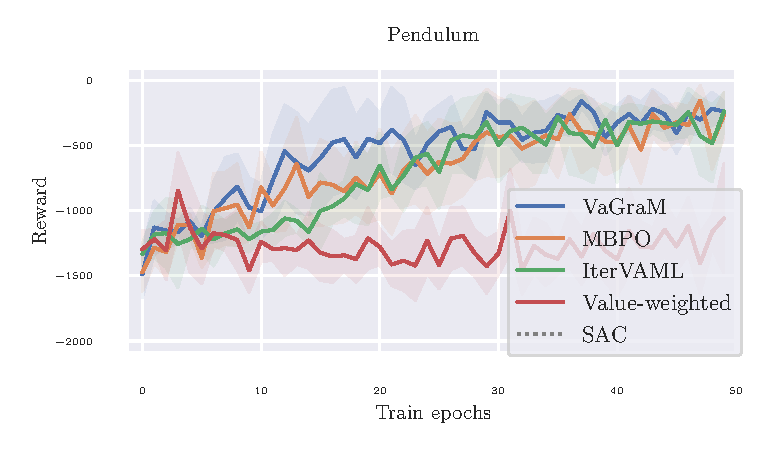
\includegraphics[width=\textwidth]{figures/vagram/pendulum_all.pdf}
\end{minipage}~
\begin{minipage}{.48\textwidth}
    \centering
    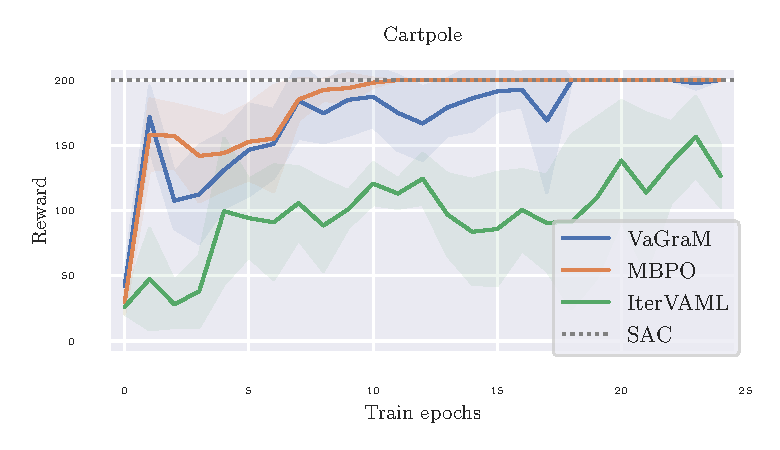
\includegraphics[width=\textwidth]{figures/vagram/cartpole.pdf}
\end{minipage}
    \caption{Comparison of VaGraM, MLE \ac{mbpo} baseline), IterVAML \textcite{itervaml} and a value-weighing ablation on two simple continuous control tasks. The shaded area represents standard error estimated over 8 runs. While VaGraM, IterVAML and \ac{mbpo} are able to achieve satisfactory performance on the Pendulum Swingup task, IterVAML fails to stabilize the more difficult Cartpole balancing task.}
    \label{fig:ablations}
\end{figure}

To test the performance of VaGraM and \ac{mbpo} against alternative models, we used the classic Pendulum swingup and Cartpole benchmarks.
As points of comparison, we used IterVAML \parencite{itervaml} and a simple value-weighted regression similar to \textcite{nair2020goal}, where the MSE error is multiplied by the inverse of the value function of the sample. The results are visualized in \autoref{fig:ablations}.
Hyperparameters follow the Cartpole task baseline in \textcite{pineda2021mbrl}.

Since IterVAML suffers from strong destabilization on the Pendulum model learning problem, as discussed in \autoref{sec:vagram:experiments}, we added an MSE loss to the original formulation $\mathcal{L}_\text{joint} = \mathcal{L}_\text{IterVAML} + \lambda \mathcal{L}_\text{MSE}$ with a tradeoff factor of $\lambda = 0.01$.
We see that this is sufficient to stabilize the performance in the Pendulum swingup task and prevent catastrophic divergence, but the model still performs significantly below the \ac{mbpo} and VaGraM results in the Cartpole stabilization task.
This is evidence that even with additional stabilization mechanisms, the issues presented in \autoref{sec:method} prevents the easy adoption of IterVAML to complex domains.

The value-weighing baseline is unable to achieve satisfactory performance even on the simple pendulum task, leading us to conclude that more complex reweighing schemes such as VaGraM are indeed necessary.

\subsection{Performance in Mujoco benchmark suite}
\begin{figure}[t]
\begin{center}
\begin{minipage}{.49\textwidth}
    \centering
    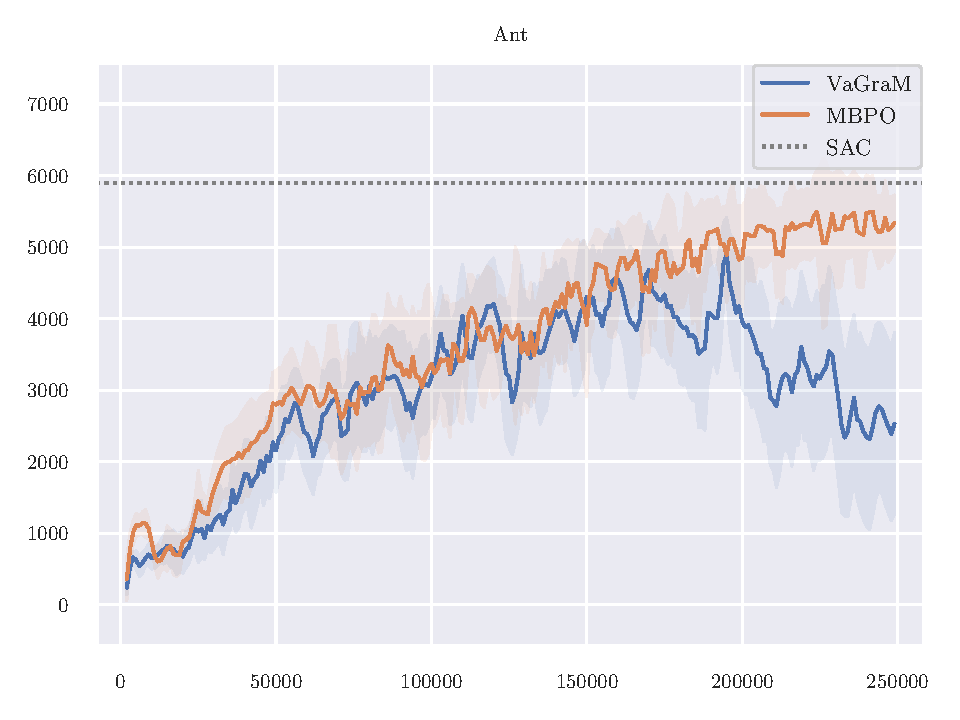
\includegraphics[width=\textwidth]{figures/vagram/ant_nonorm.pdf}
\end{minipage}~
\begin{minipage}{.49\textwidth}
    \centering
    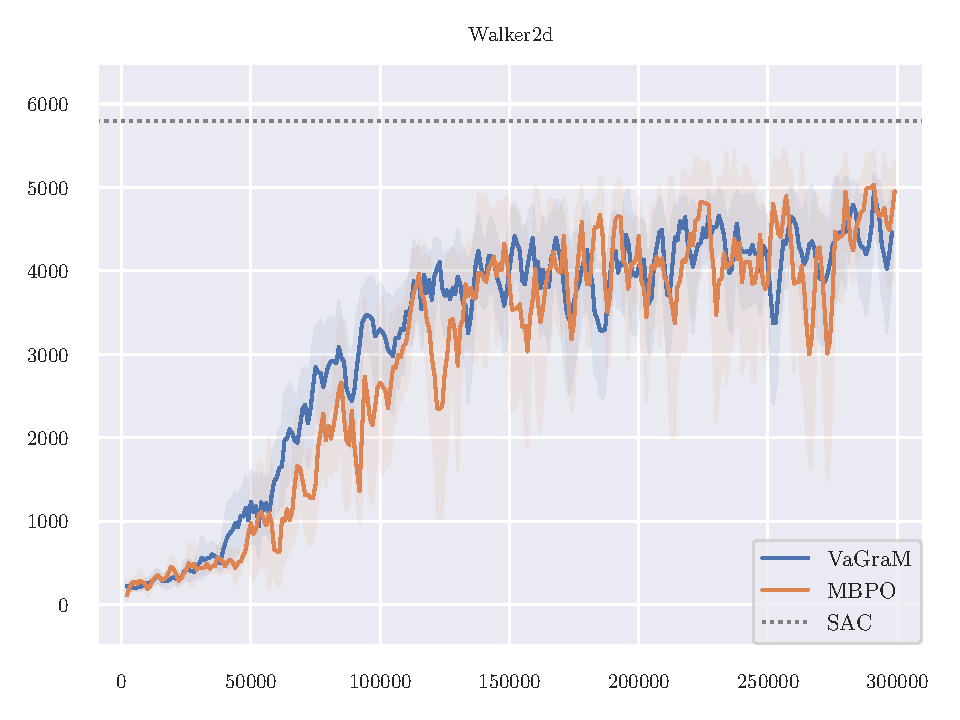
\includegraphics[width=\textwidth]{figures/vagram/walker_nonorm.pdf}
\end{minipage}
\end{center}

\begin{center}
\begin{minipage}{.49\textwidth}
    \centering
    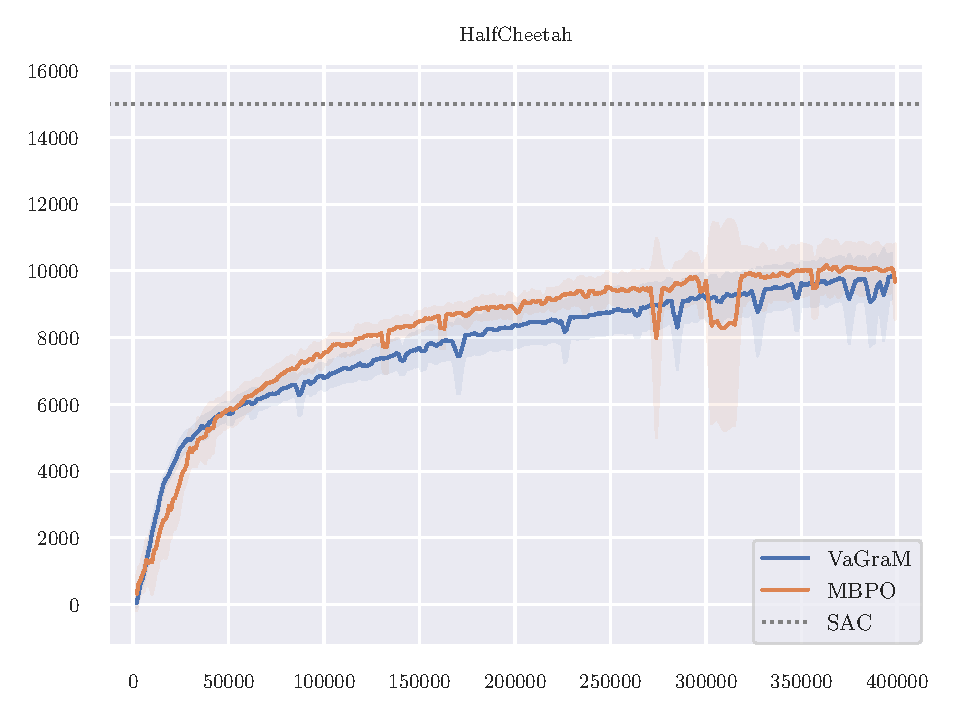
\includegraphics[width=\textwidth]{figures/vagram/cheetah_nonorm.pdf}
\end{minipage}
\end{center}
    \caption{\revised{Comparison of VaGraM and \ac{mbpo} on the Mujoco tasks presented in \textcite{mbpo}. Lines mark average performance over 8 seeds and shaded areas mark the standard error of the mean. We see that VaGraM is able to perform on par with the \ac{mbpo} implementation on the HalfCheetah and Walker tasks. It is unstable on the Ant task however.}}
    \label{fig:mujoco}
\end{figure}


In a previous version of the paper, the following experiments were faulty due to a bug in the experimental code discovered after publication.
This version includes the revised experiments.

The results of VaGraM and \ac{mbpo} are presented in \autoref{fig:mujoco}.
We find that VaGraM is able to perform on par with the \ac{mbpo} baseline on two of the remaining tasks, while not performing well on Ant.
Due to stability issues, the Humanoid-v2 task is excluded, no algorithm achieved satisfactory performance (compare \textcite{pineda2021mbrl} for a discussion). 

On the Ant task, a manual inspection of the gradients of the value function reveals that they vary across different data points very strongly.
We therefore hypothesize that the VaGraM objective can destabilize if confronted with very sharp value function gradients and requires additional regularization in challenging tasks.
To test this hypothesis, we adapt the normalization method from \textcite{bjorck2022is}.
The results are visualized in \autoref{fig:norm_mujoco}.

As is apparent from the results, the issue of destabilization on the Ant task is solved using the normalization, but it is not a panacea, as the performance on HalfCheetah suffers heavily. 
It is likely that the HalfCHeetah environment is now over-regularized which would explain the lack of performance with \ac{mbpo} as well. Overall these additional experiments suggest that there is a non-trivial relationship between the observation space, value function regularization and model-based RL. 
Testing more involved normalization schemes such as those used by \textcite{bjorck2021towards} and \textcite{zheng2023is} would be a promising direction for more in-depth research.

\begin{figure}[t]
\begin{center}
\begin{minipage}{.49\textwidth}
    \centering
    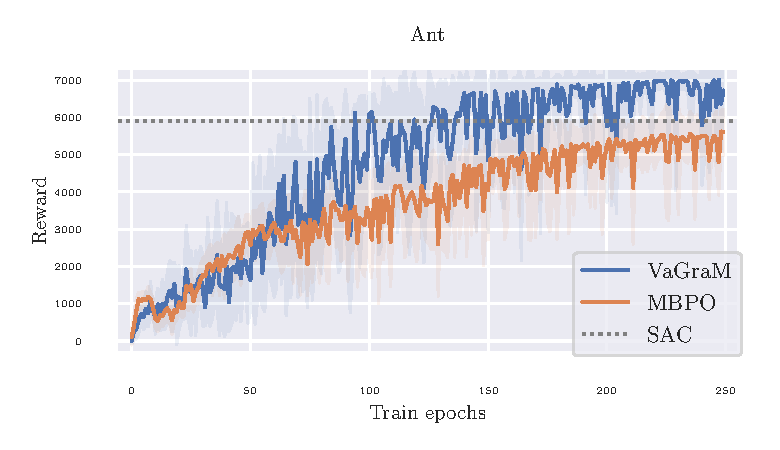
\includegraphics[width=\textwidth]{figures/vagram/ant.pdf}
\end{minipage}~
\begin{minipage}{.49\textwidth}
    \centering
    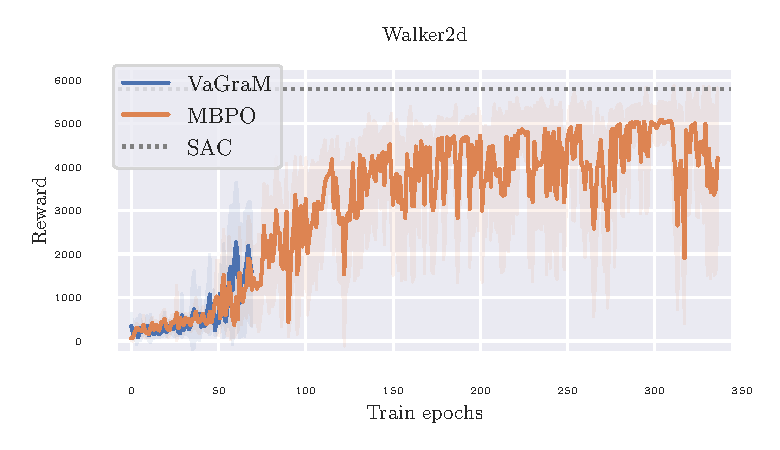
\includegraphics[width=\textwidth]{figures/vagram/walker.pdf}
\end{minipage}
\end{center}

\begin{center}
\begin{minipage}{.49\textwidth}
    \centering
    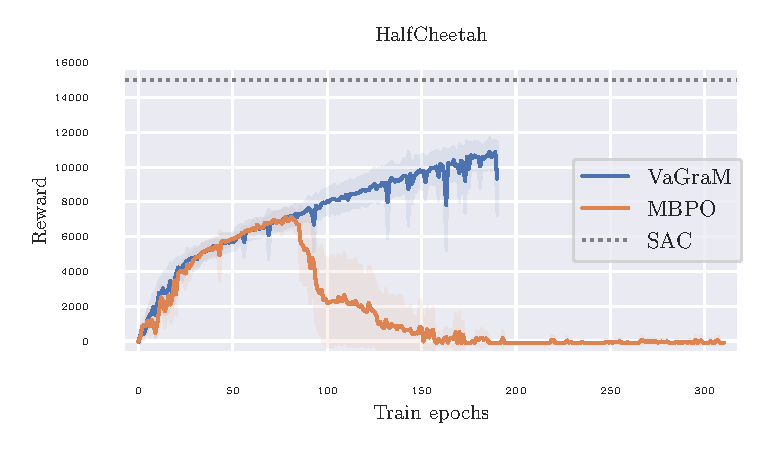
\includegraphics[width=\textwidth]{figures/vagram/cheetah.pdf}
\end{minipage}
\end{center}
    \caption{Comparison of VaGraM and \ac{mbpo} on the Mujoco tasks presented in \textcite{mbpo} using normalization \parencite{bjorck2022is}. The instability on the Ant task is solved using the normalization, but the performance on HalfCheetah and Walker2d suffers.}
    \label{fig:norm_mujoco}
\end{figure}

\section{Experiment details}
\label{app:vagram:implementation}

As described in the main paper, we conducted our experiment in two domains from the OpenAI benchmark OpenAI Gym \parencite{brockman2016openai}, Pendulum-v2 and Hopper-v0.
We used both environments as provided by the framework without further modification in our capacity tests.
Our algorithm is shown in pseudocode in \autoref{alg:vambpo}.

\paragraph{Expanded Hopper environment}
To test the performance of VaGraM in a setting with additional unnecessary state observations, we created a random dynamical system that evolves according to randomly initialized dynamics function, where $A$ is a fixed matrix with entries randomly drawn from $\mathcal{N}(0., 10.)$, and a fixed initial state $s_0$ with components randomly drawn from $\mathcal{N}(0., 0.1)$. We do not resample the fixed components at reset.

The transitions are then described by the following deterministic function:

\begin{align}
    f(s_t,a_t) &= 
  \begin{cases}
    s_t + \sin(A s) & \text{if } |f(s_t,a_t)| < 20\\
    s_0 & \text{else}
  \end{cases}
\end{align}

This dynamics function contains two attributes which are hard for neural networks to model: discontinuity and non-linear dynamics.
We find that this is sufficient to provides a very challenging environment for the MLE trained neural network models.
To account for varying difficulty over different random initialization of the environments, we made sure to test the comparison runs with the same seeds over the different loss functions, but we did not find that the inter-seed variance was larger than the observed difference between the different loss functions.

\subsection{Architecture and hyperparameters}
For the Pendulum experiments, we use a simple fully connected neural network with a single layer, and a linear model without feature transformations as architectures.
The used non-linearity is ReLU.
All experiments were implemented in PyTorch \parencite{pytorch} and were not specified, the standard initialization of the library were kept.
The exact versions of all used libraries are documented in the provided source code.

To assure a fair comparison we used the hyperparameters provided by \textcite{mbpo} for all experiments with our approach and the NLL loss function used for the baseline.
All models used were fully connected neural networks with SiLU non-linearities and standard initialization.
For all experiments with full model size we followed \ac{mbpo} and used seven ensemble members with four layers and 200 neurons per layer.

Even though our loss derivation does not support rolling out the model for more than a single step without accounting for this in the training setup, we find that VaGraM is still stable over the short rollout horizons used by \ac{mbpo}.
Therefore we used the rollout scheme from \ac{mbpo}.

However, it was necessary to make a small alteration to the training setup: in the provided implementation, the value function is solely trained on model samples.
Since our model is directly dependent on the value function, we need to break the inter-dependency between model and value function in the early training iterations.
Hence, we used both real environment data and model data to train the value function, linearly increasing the amount of model samples from 0 to 95\% of the SAC replay buffer over the first 40 epochs of training (40.000 real environment steps).
We did not transition to fully using model data to ensure that real environment samples are still able to inform the value function learning.
We found that this did not diminish the returns of \ac{mbpo} compared to solely using model samples and so used this approach for both VaGraM and MLE.

To estimate the gradient of the value function, we used the four empirical value functions, two direct estimates and two target value functions used in the SAC algorithm and summed the losses using each data tuple and value function gradient independently.
Furthermore we calculated the $L_2$ norm of all value function gradients and clipped these at the 95-th percentile.
We found that this was necessary since the empirical value function gradients can become very large, which in some cases leads to a destabilization of the gradient descent algorithm used to update the model.
Even then, in the Ant environment this is insufficient to prevent destabilization.


\begin{algorithm}[t]
\caption{Value-Gradient weighted Model learning (VaGraM)}\label{alg:vambpo}
Initialize policy $\pi_\phi$, value function $v_\psi$, model $\hat{f}_\theta$, environment dataset $\mathcal{D}_\text{env}$, model dataset $\mathcal{D}_\text{model}$\;
\For{$N$ epochs}
{
    \While{$\hat{p}_\theta$ not converged}{
        Sample batch $(s,a,r,s')$ from $\mathcal{D}_\text{env}$\;
        $\mathcal{L}_{v_\psi} = \left((s' - \hat{f}_\theta(s,a))^\intercal\text{diag}\left(\frac{d}{ds}v_\psi(s)|_{s'}\right)^2 (s' - \hat{f}_\theta(s,a))\right)$\;
        $\theta \gets \theta - \alpha \frac{d}{d \theta} \mathcal{L}_{v_\psi}$\;
        Train reward model
    }
    \For{$E$ steps}{
    Take action in env according to $\pi_\phi$; add to $\mathcal{D}_\text{env}$\;
    \For{M model rollouts}{
        Sample $s$ from $\mathcal{D}_\text{env}$; sample $a \sim \pi_\phi(s)$\;
        $s', r = \hat{f}_\theta(s,a)$\;
        Add $(s,a,r,s')$ to $\mathcal{D}_\text{model}$
    }
    \For{G policy gradient updates}{
        Sample batch $(s,a,r,s')$ from $\mathcal{D}_\text{env} \cup \mathcal{D}_\text{model}$\;
        $\psi \gets \psi - \beta \frac{d}{d\psi} (v_\psi(s) - (r + \gamma v'(s')))^2$\;
        $\phi \gets \phi - \lambda \hat{\nabla}_\phi J(\pi_\phi, v_\psi, (s,a,r,s'))$
    }
    }
}
\end{algorithm}

\section{Deterministic vs probabilistic models}
\label{app:vagram:deterministic}

Our derivation of VaGraM lead us to the conclusion that a deterministic model was sufficient to achieve the goal of value-aware model learning in environments with small transition noise.
This insight stands in contrast to the current literature, which often claims that probabilistic models are needed to achieve optimal performance in model-based reinforcement learning.
However, there is no clear consensus among different authors whether probabilistic models are needed or if a deterministic model can be sufficient for MBRL (compare \textcite{lutter2021learning}).

Our assumption that the model can be replaced with a deterministic one relies on the assumption that the underlying model is not dominated by stochastic transitions, but is deterministic or near deterministic and unimodal. 
This follows from the requirement that the model prediction admits a small error in the mean squared error sense, otherwise the Taylor approximation does not properly capture the behavior of the value function, as a model prediction might have high likelihood under the environment and still be far away from the environment sample in a mean squared sense otherwise.
In domains where capturing the stochasticity is crucial, we have to revisit this requirement in follow up work.

Furthermore, we are operating under the assumption that the mean value function of each distribution over states can be represented as the value function of a single state prediction. 
Since value function approximations represented by neural networks are continuous, this is true in our setting due to the mean value theorem for integrals.
Implicitly due to the Taylor approximation, we also assume that this mean value lies close to or on the environment sample we obtained.
If other approximation schemes are used, this property needs to be checked and potentially probabilistic models are needed to represent the expectation over all possible value functions and transition dynamics.

\subsection{Ablation experiment with deterministic models}
\begin{figure}[t]
    \centering
\begin{minipage}{.48\textwidth}    
    \centering
        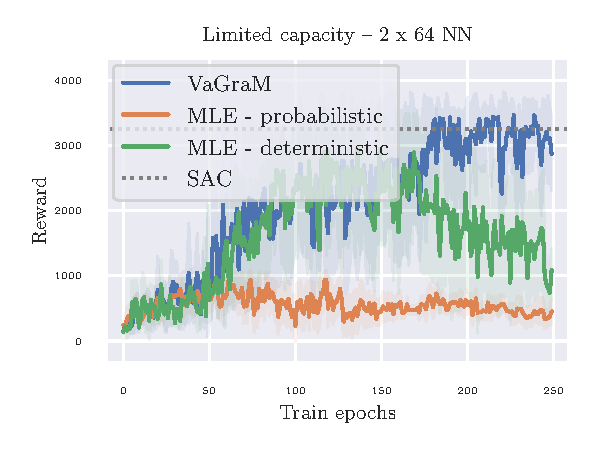
\includegraphics[width=1\linewidth]{figures/vagram/fig_3.pdf}
\end{minipage}
~
\begin{minipage}{.48\textwidth}
    \centering
        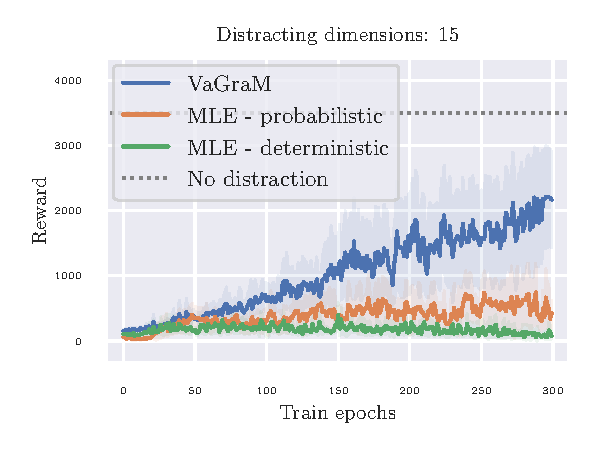
\includegraphics[width=1\linewidth]{figures/vagram/hopper_distraction_ablation.pdf}
\end{minipage}
    \caption{\textbf{Comparison of the empirical performance of deterministic and probabilistic MLE models vs VaGraM}. Thick lines denote the mean and shaded area the standard error over 8 runs. In the limited capacity setting, the deterministic model is able to achieve significantly higher returns than the probabilistic baseline, however with stability issues during longer training. On the distracting benchmark, the deterministic model is not able to achieve any significant returns.}
    \label{fig:deterministic_experiment}
\end{figure}

In our experiments in the Hopper domain, we used probabilistic models following \textcite{mbpo}. 
To verify that the improvement in performance did not result from using a deterministic model instead of a probabilistic model, we repeated the experiment showing the impact of smaller model sizes, and replaced the probabilistic Gaussian ensemble with an ensemble of deterministic functions trained with the mean squared error loss between sample and state prediction.
All other implementation details, architecture and hyperparameters were kept fixed. The results are shown in \autoref{fig:deterministic_experiment}.
In this ablation, we do indeed see that a mean squared trained model capture the dynamics information better than a model that is trained using negative log likelihood.
To the best of our knowledge, this phenomenon has not received attention in the literature, but we hypothesize that it is an artifact of training a probabilistic model with gradient descent instead of natural gradient descent (compare Figure 1 in \textcite{peters2008natural} for a visual intuition).

Nonetheless, VaGraM is still able to achieve higher cumulative reward consistently than the MSE model. 
Especially on the distraction task we find that a deterministic MSE model performs on par with the probabilistic model and fails to achieve any reward when faced with a challenging number of distractions. 
This validates our hypothesis that value awareness is important in settings with insufficient model capacity, but crucial in cases where the environment observations are not aligned with the control problem.

